\section{Methodology}
\label{sec:methodology}

\begin{figure}[t]
	\centering
	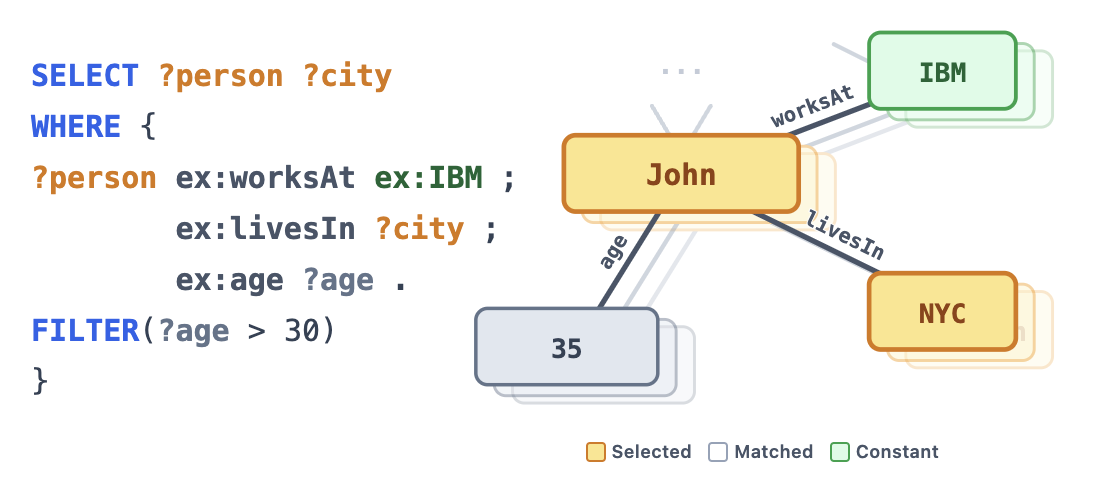
\includegraphics[width=\columnwidth]{figures/sparql.png}
	\captionsetup{skip=4pt}
	\caption{Correspondence between a SPARQL query and its matched knowledge graph subgraph.}
	\label{fig:sparql-subgraph}
\end{figure}

The central observation underlying QueryBloom is that every SPARQL query implicitly specifies a subgraph pattern over the knowledge graph (Figure~\ref{fig:sparql-subgraph}). The triple patterns in a \texttt{WHERE} clause define nodes and labeled edges that must be matched in the graph, while \texttt{SELECT} projects specific variables, and \texttt{FILTER} imposes value constraints. Each returned result row corresponds to a distinct embedding of this pattern in the graph data: a concrete assignment of entities to the query's variables that satisfies all structural and value constraints. The same argument applies to other SPARQL query forms (\texttt{ASK}, \texttt{CONSTRUCT}), which rely on the same \texttt{WHERE} clause pattern matching mechanism.

QueryBloom inverts this correspondence: it first discovers structurally diverse subgraph patterns from the knowledge graph and then jointly synthesizes SPARQL queries and natural language questions grounded in those patterns (Figure~\ref{fig:querybloom-pipeline}).

\begin{figure}[t]
	\centering
	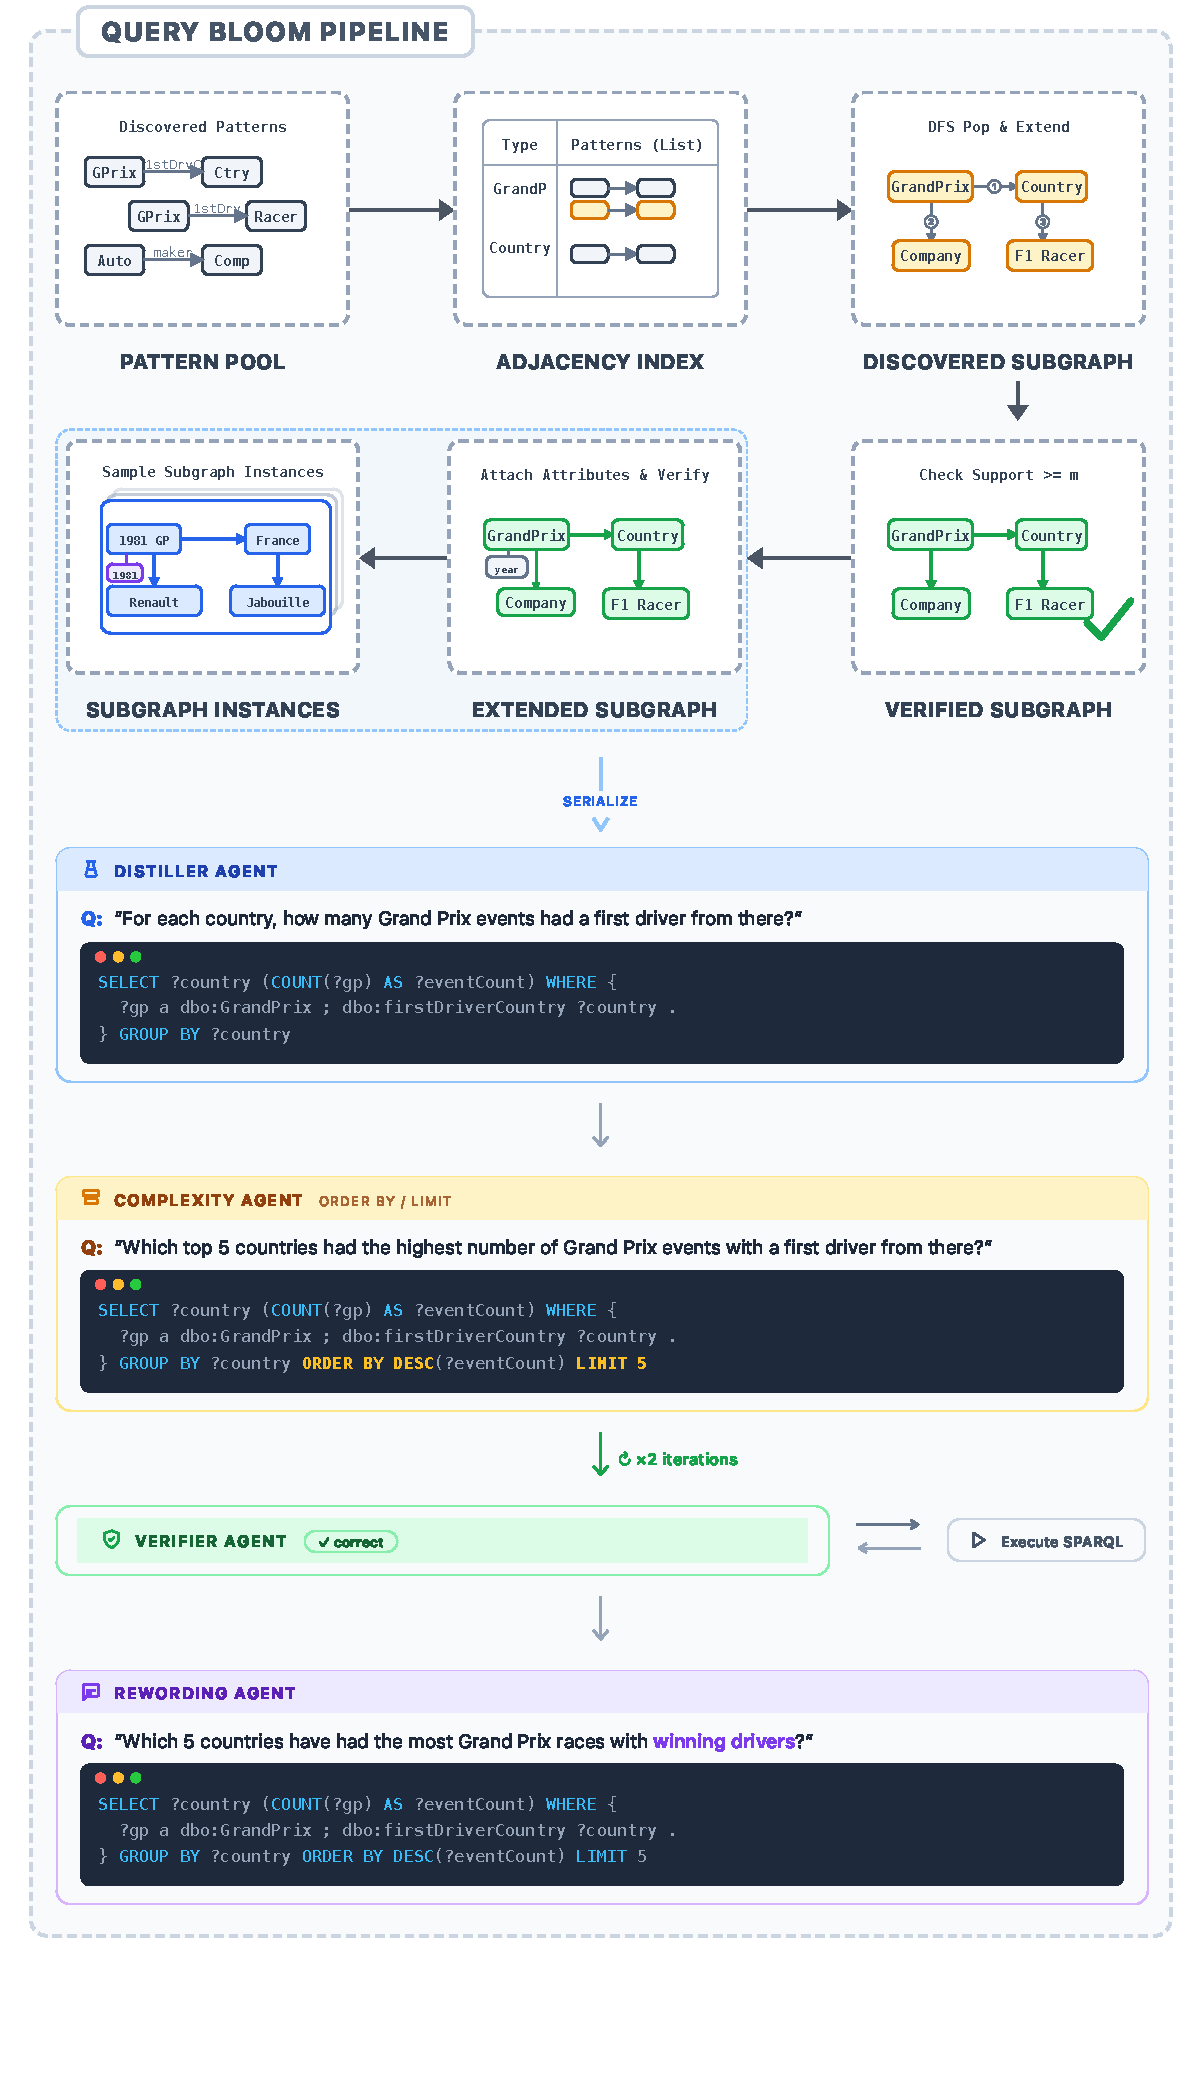
\includegraphics[width=\columnwidth,trim=0 70bp 0 0,clip]{figures/QB-Col.pdf}
	\captionsetup{skip=4pt}
	\caption{Overview of the QueryBloom methodology.}
	\label{fig:querybloom-pipeline}
\end{figure}

The pipeline proceeds through the multiple stages described below, which trace how a single subgraph pattern is discovered, grounded, and distilled into a small set of text-SPARQL pairs. The framework relies on the minimal assumption that the target knowledge graph follows W3C RDFS standards for defining classes, which is a common practice in almost all RDF knowledge graphs.

\subsection{Pattern Discovery and Adjacency Indexing}

The pipeline begins by extracting \textit{frequent type patterns} from a
property scope chosen for the target knowledge graph, adapting the ABSTAT
algorithm~\cite{Spahiu2016ABSTATOL} for efficient pattern extraction over RDF
graphs. A type pattern is a triple $(\textit{SubjectType},\;\textit{Predicate},
\;\textit{ObjectType})$ encoding that a given property connects instances of one
type to instances of another (e.g., \texttt{Person} --\texttt{worksAt} --\texttt{Organization}); patterns are discovered by sampling a large set of
triples for each property and resolving the \texttt{rdf:type} of their subject
and object nodes.

QueryBloom supports two preprocessing modes that differ in how the property
scope is determined. \textit{Whole-graph mode}, suited to smaller knowledge
graphs, enumerates all properties via a SPARQL query, removes common metadata
predicates such as labels and identifiers, and extracts patterns from the
resulting set. \textit{Online-graph mode}, suited to large graphs, begins from a
single user-specified seed property, extracts its type patterns, and then
iteratively selects properties connected to already-discovered types, adding
their patterns until a configurable property budget is reached.

In both modes, the collected patterns are filtered by a minimum support
threshold $\sigma$; the resulting set of patterns form the structural building blocks for
subgraph construction. An adjacency index is then built over this pool, mapping
each type to every pattern in which it participates and enabling constant-time
lookup of candidate extensions during subgraph discovery.

\subsection{Subgraph Discovery}

A multi-hop subgraph pattern is grown from a single frequent pattern, which serves as a two-type seed. The seed is iteratively extended by attaching adjacent patterns from the adjacency index that share at least one type with the current subgraph. Each extension adds a new edge and may introduce new types, continuing until a subgraph with $k$ distinct types is formed. At each extension, the subgraph's support is verified via a SPARQL \texttt{COUNT} query and the extension is discarded if it causes the subgraph's support to fall below the threshold $\sigma$. It follows that the subgraph will contain at least $k-1$ properties and may be cyclic or acyclic.

Once a k-type subgraph is formed, it is enriched in two further steps. First, data attributes are sampled from the discovered attribute patterns and attached to the subgraph's types and verified. Second, $m$ concrete entity instances per type that jointly satisfy the subgraph's type and property constraints are fetched from the endpoint, along with their attribute values. The subgraph comprises the abstract subgraph pattern and grounding instances with real entity URIs, labels, and attribute values to inform realistic question generation.


\subsection{LLM-Driven Text-SPARQL Distillation}

Each verified subgraph is processed by a four-stage multi-agent system whose collective purpose is to distill the subgraph into a small set of high-quality, execution-verified text-SPARQL pairs. The four agents — a \textit{generator}, a \textit{complexity introducer}, a \textit{verifier}, and a \textit{reword auditor} — operate in sequence, each receiving the subgraph as a structured YAML representation. All agents use structured output with enforced JSON schemas to guarantee perfectly parseable responses \cite{openai2024structured}.

\paragraph{Generation.}
The generator agent first assesses whether the subgraph pattern admits meaningful questions about the knowledge graph, exiting early if not. If meaningful, it generates a set of text-SPARQL pairs grounded in the subgraph's classes, entities, relationships, and attributes (see Appendix~\ref{sec:appendix_prompt}). Each generated SPARQL query is immediately executed against the endpoint, and its results are recorded alongside the pair.

\paragraph{Complexity Introduction.}
To ensure that generated question–query pairs match the complexity of real-world examples, a
\textit{complexity introducer} agent rewrites each successfully executed pair to meaningfully incorporate
additional non-trivial constructs drawn from a predefined set: value filtering, optional matching,
set union, sorting and limiting, existential checks, nested subqueries, and recursive relationships. Both the SPARQL query and its corresponding natural language question are rewritten
consistently to reflect the introduced construct. Where no meaningful augmentation is possible,
the agent skips the pair and retains the original. Every augmented query is re-executed against
the endpoint to update the execution results.

\paragraph{Verification.}
Although grounding generation in a concrete subgraph pattern is in principle sufficient to produce accurate text-SPARQL pairs (Section~\ref{sec:methodology}), an LLM is still prone to hallucination or innovation while forming the text-SPARQL. An iterative verifier agent therefore inspects every pair. Given the subgraph pattern and each pair's question, query, and execution results, the verifier judges each pair as \textit{correct} or \textit{needs-fix}. For pairs it deems in need of fixing, it additionally produces corrected question and query texts; the corrected queries are re-executed and the updated pairs are fed back into the next verification round. The loop runs for up to a configurable number of iterations or until all pairs are marked correct.

\paragraph{Question Rewording.}
As a final step, a reword agent audits the natural language question of each correct pair for KG-specific terminology leakage — such as exposed URI fragments, ontology class names, or other non-natural phrasings — and rewrites only the question text of flagged pairs, leaving the SPARQL query unchanged.

All four LLM calls operate with high reasoning effort to maximise correctness, and only pairs that pass verification are retained in the final dataset.

\subsection{Design Principles}

The pipeline is designed to produce a text-SPARQL example set that is \textit{comprehensive}, \textit{diverse}, and of \textit{high quality}.

\paragraph{Comprehensiveness.} The overall algorithm orchestrates the stages described above by seeding at least one subgraph from every frequent type pattern in the constructed pool. Thus, coverage is defined with respect to the chosen preprocessing mode: whole-graph mode covers all frequent patterns found among the graph's selected non-metadata properties, whereas online graph mode covers all frequent patterns found for the seed property and any connected properties added within the property budget. As opposed to graph mining, we deliberately adopt a very low support threshold because even rare subgraph patterns can give rise to meaningful questions.


\paragraph{Diversity.} Several mechanisms ensure diversity in the generated examples: (i) unlike a random walk that follows a linear path, the subgraph is extended by selecting a new pattern from \textit{any type} contained in the current subgraph, producing diverse structural compositions; (ii) the target number of types $k$ is sampled from a range distribution to produce subgraphs of varying sizes; (iii) for each subgraph, we randomly sample $v$ attributes per class to ensure diverse coverage of class attributes; (iv) the distiller agent is prompted to produce variations in question and query style, covering different query patterns (e.g., \texttt{SELECT}, aggregation, \texttt{ASK}, \texttt{FILTER}, \texttt{OPTIONAL}, \texttt{GROUP BY}).

\paragraph{Quality.} Quality is safeguarded at multiple stages. Subgraphs that are trivial or concern only graph metadata are flagged as non-meaningful during generation and excluded. The generate-execute-verify loop ensures that every retained pair produces results expected by the distiller agent. The distiller agent's core objective is to elicit questions from the subgraph that a domain expert would be expected to ask.

\FloatBarrier